\documentclass[12pt]{article}
\usepackage{graphicx}
\usepackage{enumitem}
\usepackage{multicol}
\usepackage{mathtools}
\usepackage{hyperref}
\usepackage[margin=1in]{geometry}
\usepackage{amsmath,amsthm,amssymb}
\usepackage[makeroom]{cancel}

 
\begin{document}

%\begin{equation*}
%\begin{split}
    
%\end{split}
%\end{equation*}
 
% --------------------------------------------------------------
%                         Start here
% --------------------------------------------------------------
 
\title{AST1430 Assignment 4}
\author{Jessica Campbell}
\date{April 3, 2018}
\maketitle

% --------------------------------------------------------------
%     1. Thermal Bremsstrahlung and Temperature of a HII region
% --------------------------------------------------------------

\section{Thermal Bremsstrahlung and Temperature of an $\mathrm{HII}$ region}

The 3rd problem of Problem set 4 in Frank Shu’s ``The physics of astrophysics'', except for the last paragraph.

% --------------------------------------------------------------
%               Part 1
% --------------------------------------------------------------

\section*{Part 1}

In this problem, we consider how radio observations of free-free emission provide diagnostics of the physical conditions of $\mathrm{HII}$ regions. (Analogous considerations apply to X-ray observations of hot gas in galaxy clusters.) Assume an $\mathrm{HII}$ region to have a uniform electron temperature $T$ and density $n_e$ which we would like to determine by observational means.

Since the free-free emission associated with thermal distribution of electron occurs under condition of LTE, satisfy yourself that Equation \ref{eq:1} of the text yields the solution for the equation of transfer:

\begin{align} \label{eq:1}
I_\nu = I_\nu(0)e^{-\tau_\nu}+B_\nu(T)(1-e^{-\tau_\nu}).
\end{align}

% --------------------------------------------------------------
%               Solution
% --------------------------------------------------------------

\subsection*{Solution}



% --------------------------------------------------------------
%               Part 2
% --------------------------------------------------------------

\section*{Part 2}

For radio observations spanning, say, $\lambda \sim 100\,\mathrm{cm}$ to $1\,\mathrm{mm}$, show that $h\nu \ll k_BT$ for all likely values of $T$. Thus it represents a good approximation to replace $B_\nu(T)$ by its Rayleigh-Jeans limit:

\begin{align*}
{\rm Rayleigh\,-\, Jeans:}~~~~~B_\nu(T)=\frac{2\nu^2}{c^2}k_BT.
\end{align*}

Motivated by this simplification, radio astronomers then like to express the specific intensity $I_\nu$ in terms of a \textit{brightness temperature} $T_b$ defined through 

\begin{align} \label{eq:2}
T_b \equiv \frac{c^2}{2\nu^2k}I_\nu.
\end{align}

Show now that Equation \ref{eq:1} can be rewritten as 

\begin{align} \label{eq:3}
T_b = T_b(0)e^{-\tau_\nu} +T\,(1-e^{-\tau_\nu}),
\end{align}

{\noindent}which applies not only to free-free radiation, but whenever (a) we may ignore the effects of scattering, and (b) we may assume that the source function has an LTE value at a uniform temperature $T$ throughout the region being observed. (Notice that we have not yet assumed uniformity of density.)

% --------------------------------------------------------------
%               Solution
% --------------------------------------------------------------

\subsection*{Solution}

For radio observations spanning $\lambda \sim 100\,\mathrm{cm}$ to $\lambda \sim 1\,\mathrm{mm}$, we can calculate the respective range of photon energies via $k_BT$ assuming a typical $\mathrm{HII}$ temperature of $10^4\,\mathrm{K}$. The minimum energy of this range will be 

\begin{align*}
    E_\mathrm{min} = h\nu_\mathrm{min} = \frac{hc}{\lambda_\mathrm{max}} = \frac{hc}{100\,\mathrm{cm}} = 1.2\times10^{-6}\,\mathrm{eV}
\end{align*}

{\noindent}while the maximum will be

\begin{align*}
    E_\mathrm{max} = h\nu_\mathrm{max} = \frac{hc}{\lambda_\mathrm{min}} = \frac{hc}{1\,\mathrm{mm}} = 1\times10^{-3}\,\mathrm{eV}.
\end{align*}

{\noindent}Assuming a typical $\mathrm{HII}$ temperature of $10^4\,\mathrm{K}$, the energy of the free-free emission is given by

\begin{align*}
    k_BT = k_B\,10^4\,\mathrm{K} = 0.86\,\mathrm{eV}.
\end{align*}

{\noindent}Therefore, across the range of radio photon energies of $1.2\times10^{-6}\,\mathrm{eV}$ -- $1\times10^{-3}\,\mathrm{eV}$, it holds that $h\nu \ll k_BT$.

Defining a \textit{brightness temperature} as 

\begin{align*}
    T_b \equiv \left( \frac{c^2}{2\nu^2k_B} \right) I_\nu,
\end{align*}

{\noindent}the specific intensity $I_\nu$ can be written as:

\begin{align*}
    I_\nu = \left( \frac{2\nu^2k_B}{c^2} \right) T_b.
\end{align*}

{\noindent}Substituting this into the equation of radiative transfer yields

\begin{equation*}
\begin{split}
    \frac{d}{d\tau_\nu} (I_\nu) &= S_\nu - I_\nu \\
    \frac{d}{d\tau_\nu} \left( \frac{2\nu^2k_B}{c^2} \right) T_b &= S_\nu - \left( \frac{2\nu^2k_B}{c^2} \right) T_b.
\end{split}
\end{equation*}

{\noindent}For thermal emission, the source function equals the Planck function which satisfies the following approximation in the Rayleigh-Jeans limit:

\begin{equation*}
\begin{split}
    S_\nu &= B_\nu(T) \\
    B_\nu(T) &= \frac{2h\nu^3}{c^2} \frac{1}{\exp\left(\frac{\Delta E}{k_BT}\right) - 1} \\
    B_\nu(T) &\approx \frac{2h\nu^3}{c^2} \frac{1}{\left(1 + \frac{\Delta E}{k_BT}\right) - 1} \\
    B_\nu(T) &\approx \frac{2h\nu^3}{c^2} \frac{1}{\left(\frac{\Delta E}{k_BT}\right)} \\
    B_\nu(T) &\approx \frac{2h\nu^3}{c^2} \frac{k_BT}{\Delta E} \\
    B_\nu(T) &\approx \frac{2h\nu^3}{c^2} \frac{k_BT}{h\nu} \\
    B_\nu(T) &\approx \frac{2\cancel{h}\nu^{\cancel{3}2}}{c^2} \frac{k_BT}{\cancel{h}\cancel{\nu}} \\
    B_\nu(T) &\approx \left(\frac{2\nu^2k_B}{c^2}\right) T.
\end{split}
\end{equation*}

{\noindent}Making this substitution for the source function $S_\nu$ in the equation of radiative transfer yields

\begin{equation*}
\begin{split}
    \frac{d}{d\tau_\nu} \left( \frac{2\nu^2k_B}{c^2} \right) T_b &= \left(\frac{2\nu^2k_B}{c^2}\right) T - \left( \frac{2\nu^2k_B}{c^2} \right) T_b \\
    \cancel{\left( \frac{2\nu^2k_B}{c^2} \right)} \frac{d}{d\tau_\nu} T_b &= \cancel{\left(\frac{2\nu^2k_B}{c^2}\right)} T - \cancel{\left( \frac{2\nu^2k_B}{c^2} \right)} T_b \\
    \frac{dT_b}{d\tau_\nu} &= T - T_b.
\end{split}
\end{equation*}

{\noindent}Solving the linear differential equation while making the substitution $x\equiv T-T_b$

\begin{equation*}
\begin{split}
    \frac{dT_b}{d\tau_\nu} &= T - T_b \\
    \frac{dT_b}{T - T_b} &= d\tau_\nu \\
    \int_{T-T_b(0)}^{T-T_b}\frac{dT_b}{T - T_b} &= \int_0^{\tau_\nu}d\tau_\nu \\
    \int_{T-T_b(0)}^{T-T_b}\frac{-dx}{x} &= \int_0^{\tau_\nu}d\tau_\nu \\
    \int_{T-T_b(0)}^{T-T_b}\frac{dx}{x} &= -\int_0^{\tau_\nu}d\tau_\nu \\
    \ln(x)\rvert_{T-T_b(0)}^{T-T_b} &= -\tau_\nu\rvert_0^{\tau_\nu} \\
    \ln(T-T_b) - \ln(T-T_b(0)) &= -\tau_\nu \\
    \ln\left(\frac{T-T_b}{T-T_b(0)}\right) &= -\tau_\nu \\
    \exp\left\{\ln\left(\frac{T-T_b}{T-T_b(0)}\right)\right\} &= \exp(-\tau_\nu) \\
    \left(\frac{T-T_b}{T-T_b(0)}\right) &= e^{-\tau_\nu} \\
    T-T_b &= (T-T_b(0))e^{-\tau_\nu} \\
    T_b &= T - (T-T_b(0))e^{-\tau_\nu} \\
    T_b &= T_b(0)e^{-\tau_\nu} + T(1-e^{-\tau_\nu}).
\end{split}
\end{equation*}

{\noindent}This yields the desired solution for the brightness temperature $T_b$:

\begin{align*}
    \boxed{T_b = T_b(0)e^{-\tau_\nu} + T(1-e^{-\tau_\nu})}.
\end{align*}

% --------------------------------------------------------------
%               Part 3
% --------------------------------------------------------------

\section*{Part 3}

Applied to free-free emission, $\tau_\nu$ has the form:

\begin{align*}
\tau_\nu = \int \rho\kappa_\nu^{ff}ds,
\end{align*}

{\noindent}where the integral is taken along the line of sight throughout the $\mathrm{HII}$ region and $\rho\kappa_\nu^{ff}$ is given by equation (15.29)$^1$ of the text. Assume for simplicity a pure hydrogen plasma, expand the exponential in the correction for stimulated emission, $1-e^{-h\nu/k_BT}$, for small $h\nu/k_BT$, and show that 

\begin{align*}
\rho\kappa_\nu^{ff} =Cn_e^2T^{-3/2}\nu^{-2}\bar{g}_\nu^{ff},
\end{align*}

{\noindent}where $C$ is a constant coefficient,

\begin{align*}
C \equiv \left(\frac{2m_e}{3\pi k_B}\right)^{1/2}\left[\frac{4\pi e^6}{3m_e^2 c k_B}\right].
\end{align*}

$^1$ Equation (15.29) is 

\begin{align*}
\rho\kappa_\nu^{ff} = \sum n(Z_i)n_e\left(\frac{2m_e}{3\pi k_BT}\right)^{1/2}\left[\frac{4\pi Z_i^2e^6}{3m_e^2ch\nu^3}\right]\bar{g}_\nu^{ff}(\nu)\left(1-e^{-h\nu/k_BT}\right).
\end{align*}

% --------------------------------------------------------------
%               Solution
% --------------------------------------------------------------

\subsection*{Solution}

For free-free emission, $\rho\kappa_\nu^{ff}$ has the form

\begin{align*}
    \rho\kappa_\nu^{ff} = \sum n(Z_i)n_e\left(\frac{2m_e}{3\pi k_BT}\right)^{1/2}\left[\frac{4\pi Z_i^2e^6}{3m_e^2ch\nu^3}\right]\bar{g}_\nu^{ff}(\nu)\left(1-e^{-h\nu/k_BT}\right).
\end{align*}

{\noindent}Assuming a pure hydrogen plasma, the atomic mass number $Z_i\equiv1$ so $\sum n(Z_i)=n_e$ and $h\nu/k_BT\ll1$, and re-writing in a form that allows us to collect terms for $C$,

\begin{equation*}
\begin{split}
    \rho\kappa_\nu^{ff} &= \sum n(Z_i)n_e\left(\frac{2m_e}{3\pi k_BT}\right)^{1/2}\left[\frac{4\pi Z_i^2e^6}{3m_e^2ch\nu^3}\right]\bar{g}_\nu^{ff}(\nu)\left(1-e^{-h\nu/k_BT}\right) \\
    \rho\kappa_\nu^{ff} &= (n_e)n_e\left(\frac{2m_e}{3\pi k_BT}\right)^{1/2}\left[\frac{4\pi (1)^2e^6}{3m_e^2ch\nu^3}\right]\bar{g}_\nu^{ff}(\nu)\left(1-e^{-h\nu/k_BT}\right) \\
    \rho\kappa_\nu^{ff} &= n_e^2\left(\frac{2m_e}{3\pi k_BT}\right)^{1/2}\left[\frac{4\pi e^6}{3m_e^2ch\nu^3}\right]\bar{g}_\nu^{ff}(\nu)\left(1-e^{-h\nu/k_BT}\right) \\
    \rho\kappa_\nu^{ff} &= n_e^2\left(\frac{2m_e}{3\pi k_B}\right)^{1/2} \left(\frac{1}{T}\right)^{1/2}\left[\frac{4\pi e^6}{3m_e^2ck_B}\right] \left[\frac{k_B}{h\nu^3}\right]\bar{g}_\nu^{ff}(\nu)\left(1-e^{-h\nu/k_BT}\right) \\
    \rho\kappa_\nu^{ff} &= \left(\frac{2m_e}{3\pi k_B}\right)^{1/2} \left[\frac{4\pi e^6}{3m_e^2ck_B}\right]n_e^2 \left(\frac{1}{T}\right)^{1/2} \left[\frac{k_B}{h\nu^3}\right]\bar{g}_\nu^{ff}(\nu)\left(1-e^{-h\nu/k_BT}\right) \\
    \rho\kappa_\nu^{ff} &= \left\{\left(\frac{2m_e}{3\pi k_B}\right)^{1/2} \left[\frac{4\pi e^6}{3m_e^2ck_B}\right]\right\} n_e^2 T^{-1/2} \left[\frac{k_B}{h\nu^3}\right]\bar{g}_\nu^{ff}(\nu)\left(1-e^{-h\nu/k_BT}\right) \\
    \rho\kappa_\nu^{ff} &= C n_e^2 T^{-1/2} \left(\frac{k_B}{h\nu^3}\right)\bar{g}_\nu^{ff}(\nu)\left(1-e^{-h\nu/k_BT}\right) \\
    \rho\kappa_\nu^{ff} &\approx C n_e^2 T^{-1/2} \left(\frac{k_B}{h\nu^3}\right)\bar{g}_\nu^{ff}(\nu)\left(1-(1-\frac{h\nu}{k_BT})\right) \\
    \rho\kappa_\nu^{ff} &= C n_e^2 T^{-1/2} \left(\frac{\cancel{k_B}}{\cancel{h}\nu^{\cancel{3}2}}\right)\bar{g}_\nu^{ff}(\nu)\left(\frac{\cancel{h}\cancel{\nu}}{\cancel{k_B}T}\right) \\
    \rho\kappa_\nu^{ff} &= C n_e^2 T^{-1/2} \left(\frac{1}{\nu^2}\right)\bar{g}_\nu^{ff}(\nu)\left(\frac{1}{T}\right) \\
    \rho\kappa_\nu^{ff} &= C n_e^2 T^{-1/2}T^{-1} \nu^{-2}\bar{g}_\nu^{ff}(\nu) \\
    \rho\kappa_\nu^{ff} &= C n_e^2 T^{-3/2} \nu^{-2}\bar{g}_\nu^{ff}(\nu).
\end{split}
\end{equation*}

{\noindent}This gives us the desired expression for $\rho\kappa_\nu^{ff}$:

\begin{align*}
\boxed{\rho\kappa_\nu^{ff} = C n_e^2 T^{-3/2} \nu^{-2}\bar{g}_\nu^{ff}(\nu)}.
\end{align*}

% --------------------------------------------------------------
%               Part 4
% --------------------------------------------------------------

\section*{Part 4}

The Gaunt factor $\bar{g}_\nu^{ff}$ in the radio regime reads

\begin{align*}
\bar{g}_\nu^{ff} = \frac{\sqrt3}{2\pi}\left[\ln\left(\frac{8k^3T^3}{\pi^2e^4m_e\nu^2}\right)-5\gamma\right],
\end{align*}

{\noindent}where $\gamma = 0.5772...$ is Euler's Constant. Compute $\bar{g}_\nu^{ff}$ for $\nu = 10^9$ Hz and $T = 10^4\,\mathrm{K}$, and show that, unlike the optical case, $\bar{g}_\nu^{ff}$ should not be approximated by unity here. Notice also that Planck's constant $h$ has dropped out of all the equations, so that the considerations are purely classical.

% --------------------------------------------------------------
%               Solution
% --------------------------------------------------------------

\subsection*{Solution}

The Gaunt factor in the radio regime has the form

\begin{align*}
    \bar{g}_\nu^{ff} = \frac{\sqrt3}{2\pi}\left[\ln\left(\frac{8k^3T^3}{\pi^2e^4m_e\nu^2}\right)-5\gamma\right].
\end{align*}

{\noindent}where $\gamma=0.5772...$ is Euler's constant. Computing the Gaunt factor for $\nu=10^9\,\mathrm{Hz}$ and $T=10^4\,\mathrm{K}$,

\begin{align*}
    \bar{g}_\nu^{ff} = \frac{\sqrt3}{2\pi}\left[\ln\left(\frac{8k^3(10^4\,\mathrm{K})^3}{\pi^2e^4m_e(10^9\,\mathrm{Hz})^2}\right)-5(0.5772)\right] = 5.96.
\end{align*}

Therefore,

\begin{align*}
    \boxed{\bar{g}_\nu^{ff}(\nu=10^9\,\mathrm{Hz},T=10^4\,\mathrm{K}) = 5.96}
\end{align*}

% --------------------------------------------------------------
%               Part 5
% --------------------------------------------------------------

\section*{Part 5}

Define the \textit{emission measure} as the integral

\begin{align*}
{\rm EM} \equiv \int n_e^2ds,
\end{align*}

{\noindent}and show that $\tau_\nu$ can be expressed as 

\begin{align} \label{eq:4}
\tau_\nu = ({\rm EM})CT^{-3/2}\nu^{-2}\bar{g}_\nu^{ff}.
\end{align}


{\noindent}At low frequencies, $\tau_\nu \gg 1,$ whereas at high frequencies, $\tau_\nu \ll 1$. With no background source, show that this implies $T_b \approx T$ at low frequencies, while $T_b \approx T\tau_\nu$ at high frequencies.

% --------------------------------------------------------------
%               Solution
% --------------------------------------------------------------

\subsection*{Solution}

Using the definition of emission measure $\mathrm{EM} \equiv \int n_e^2ds$ and our previously derived solution for $\rho\kappa_\nu^{ff}$,

\begin{equation*}
\begin{split}
    \tau_\nu &= \int \rho\kappa_\nu^{ff}ds \\
    \tau_\nu &= \int C n_e^2 T^{-3/2} \nu^{-2}\bar{g}_\nu^{ff}(\nu) ds \\
    \tau_\nu &= \left\{ \int n_e^2ds\right\} C T^{-3/2} \nu^{-2}\bar{g}_\nu^{ff}(\nu) \\
    \tau_\nu &= \mathrm{(EM)} C T^{-3/2} \nu^{-2}\bar{g}_\nu^{ff}(\nu).
\end{split}
\end{equation*}

{\noindent}This provides the form we are after,

\begin{align*}
    \boxed{\tau_\nu = \mathrm{(EM)} C T^{-3/2} \nu^{-2}\bar{g}_\nu^{ff}(\nu)}.
\end{align*}

Recalling our previously derived expression for the brightness temperature, the solution for no background radiation is

\begin{equation*}
\begin{split}
    T_b &= T_b(0)e^{-\tau_\nu} + T(1-e^{-\tau_\nu}) \\
    T_b &= \cancel{T_b(0)e^{-\tau_\nu}} + T(1-e^{-\tau_\nu}) \\
    T_b &= T(1-e^{-\tau_\nu}).
\end{split}
\end{equation*}

{\noindent}For low $\nu$, $\tau_\nu\gg1$ so

\begin{equation*}
\begin{split}
    T_b &= T(1-e^{-\tau_\nu}) \\
    T_b &= T(1-\cancel{e^{-\tau_\nu}}) \\
    T_b &\approx T,
\end{split}
\end{equation*}

{\noindent}which gives us the solution for $T_b(\tau_\nu\gg1)$:

\begin{align*}
    T_b(\tau_\nu\gg1) \approx T.
\end{align*}

{\noindent}For high $\nu$, $\tau_\nu\ll1$ so

\begin{equation*}
\begin{split}
    T_b &= T(1-e^{-\tau_\nu}) \\
    T_b &\approx T(1 - (1-\tau_\nu)) \\
    T_b &\approx T\tau_\nu,
\end{split}
\end{equation*}

{\noindent}giving us the solution for $T_b(\tau_\nu\ll1)$:

\begin{align*}
    T_b(\tau_\nu\ll1) \approx \tau_\nu T.
\end{align*}

Therefore,

\begin{equation*}
\boxed{ 
T_b \approx
\left\{
\begin{aligned}
T,          ~~~~~& \mathrm{if}\,\tau_\nu \gg 1 \,\mathrm{(low\,\nu)} \\
\tau_\nu T, ~~~~~& \mathrm{if}\,\tau_\nu \ll 1 \,\mathrm{(high\,\nu)}
\end{aligned}
\right.
}.
\end{equation*}

% --------------------------------------------------------------
%               Part 6
% --------------------------------------------------------------

\section*{Part 6}

For a spherical $\mathrm{HII}$ region with radius $R_S$, show that the observed flux (measured in Janskys = $10^{-26}\, {\rm watts}\,{\rm m}^{-2}\,{\rm Hz}^{-1}$ by radio astronomers) is $F_\nu = \pi I_\nu(R_S^2/r^2)$ where $r$ is the distance to the source. The size $R_S$ can be determined if the source is angularly resolved and its distance known. Show now that 

\begin{align} \label{eq:5}
F_\nu = \frac{2\pi k}{c^2}\left(\frac{R_S}{r}\right)^2 \nu^2 T_b
\end{align}

{\noindent}will be proportional to $\nu^2$ at low frequencies and to $\bar{g}_\nu^{ff}$ (a nearly flat function $\propto \nu^{-0.1}$) at high (radio) frequencies. Describe qualitatively how this information could be used to deduce $T$ and EM if the spectrum on both sides of the turnover frequency $\nu_c$ (where $\tau_\nu =1 $) can be measured. (A better way in the radio to obtain the electron temperature is to measure the strength of the ${\rm H109}\alpha$ recombination line.)

% --------------------------------------------------------------
%               Solution
% --------------------------------------------------------------

\subsection*{Solution}

Recall the definition of radiative flux:

\begin{equation*}
\begin{split}
    F_\nu &\equiv \int I_\nu \cos \theta d\Omega,
\end{split}
\end{equation*}

{\noindent}where $\theta$ is the observing angle and $d\Omega$ is the on-sky solid angle of the emitting object. Noting that the definition of solid angle is $\Omega \equiv A/r^2$:

\begin{equation*}
\begin{split}
    F_\nu &= \int_0^\infty I_\nu \int_0^\Omega \cos \theta d\Omega \\
    F_\nu &= I_\nu \cos \theta \Omega \\
    F_\nu &= I_\nu \cos(0) \left(\frac{A}{r^2}\right) \\
    F_\nu &= I_\nu \cos(0) \left(\frac{\pi R_S^2}{r^2}\right) \\
    F_\nu &= \pi I_\nu \left(\frac{R_S^2}{r^2}\right).
\end{split}
\end{equation*}

This gives us the observed flux of the $\mathrm{HII}$ region,

\begin{align*}
    \boxed{F_\nu = \pi I_\nu \left(\frac{R_S^2}{r^2}\right)}.
\end{align*}

If we recall the definition of brightness temperature,

\begin{align*}
    T_b \equiv \left(\frac{c^2}{2\nu^2k_B}\right)I_\nu,
\end{align*}

{\noindent}this allows us to write the specific intensity as

\begin{align*}
    I_\nu = \left(\frac{2\nu^2k_B}{c^2}\right)T_b.
\end{align*}

{\noindent}Plugging this into the equation for the observed flux that we just derived and rearranging terms,

\begin{equation*}
\begin{split}
    F_\nu &= \pi I_\nu \left(\frac{R_S^2}{r^2}\right) \\
    F_\nu &= \pi \left(\frac{2\nu^2k_B}{c^2}T_b\right) \left(\frac{R_S^2}{r^2}\right) \\
    F_\nu &= \frac{2\pi k_B}{c^2} \left(\frac{R_S}{r}\right)^2 \nu^2T_b.
\end{split}
\end{equation*}

This gives us the final form of flux,

\begin{align*}
    \boxed{F_\nu = \frac{2\pi k_B}{c^2} \left(\frac{R_S}{r}\right)^2 \nu^2T_b}.
\end{align*}

We previously derived that at low frequencies, $T_b \approx T$ which allows $F_\nu$ to remain proportional to $\nu^2$. At high (radio) frequencies, we also found that $T_b \approx \tau_\nu T$. We can therefore use the solution that we previously derived for optical depth,

\begin{align*}
    \tau_\nu = (\mathrm{EM})CT^{-3/2}\nu^{-2}\bar{g}_\nu^{-ff}.
\end{align*}

{\noindent}Making this substitution for $\tau_\nu$,

\begin{equation*}
\begin{split}
    F_\nu &= \frac{2\pi k_B}{c^2} \left(\frac{R_S}{r}\right)^2 \nu^2(\tau_\nu T) \\
    F_\nu &= \frac{2\pi k_B}{c^2} \left(\frac{R_S}{r}\right)^2 \nu^2 \left((\mathrm{EM})CT^{-3/2}\nu^{-2}\bar{g}_\nu^{ff}\right) T \\
    F_\nu &= (\mathrm{EM})C \frac{2\pi k_B}{c^2} \left(\frac{R_S}{r}\right)^2 \cancel{\nu}^2\cancel{\nu}^{-2} T^{-3/2}T\bar{g}_\nu^{ff}\\
    F_\nu &= (\mathrm{EM})C \frac{2\pi k_B}{c^2} \left(\frac{R_S}{r}\right)^2 \bar{g}_\nu^{ff} T^{-1/2} \\
    F_\nu &\propto \bar{g}^{ff}.
\end{split}
\end{equation*}

Therefore we have the following solutions for $F_\nu$:

\begin{equation*}
\boxed{ 
F_\nu =
\left\{
\begin{aligned}
\frac{2\pi k_B}{c^2} \left(\frac{R_S}{r}\right)^2 \nu^2T,       ~~~~~& \mathrm{if}\,\tau_\nu \gg 1 \,\mathrm{(low\,\nu)} \\
(\mathrm{EM})C \frac{2\pi k_B}{c^2} \left(\frac{R_S}{r}\right)^2 \bar{g}_\nu^{ff} T^{-1/2},~~~~~& \mathrm{if}\,\tau_\nu \ll 1 \,\mathrm{(high\,\nu)}
\end{aligned}
\right.
},
\end{equation*}

{\noindent}which provides the following proportionalities:

\begin{equation*}
\boxed{ 
F_\nu \propto
\left\{
\begin{aligned}
\nu^2,       ~~~~~& \mathrm{if}\,\tau_\nu \gg 1 \,\mathrm{(low\,\nu)} \\
\bar{g}^{ff},~~~~~& \mathrm{if}\,\tau_\nu \ll 1 \,\mathrm{(high\,\nu)}
\end{aligned}
\right.
}.
\end{equation*}


% --------------------------------------------------------------
%               Part 7
% --------------------------------------------------------------

\section*{Part 7}

\begin{figure}[h] \label{fig:P4-1}
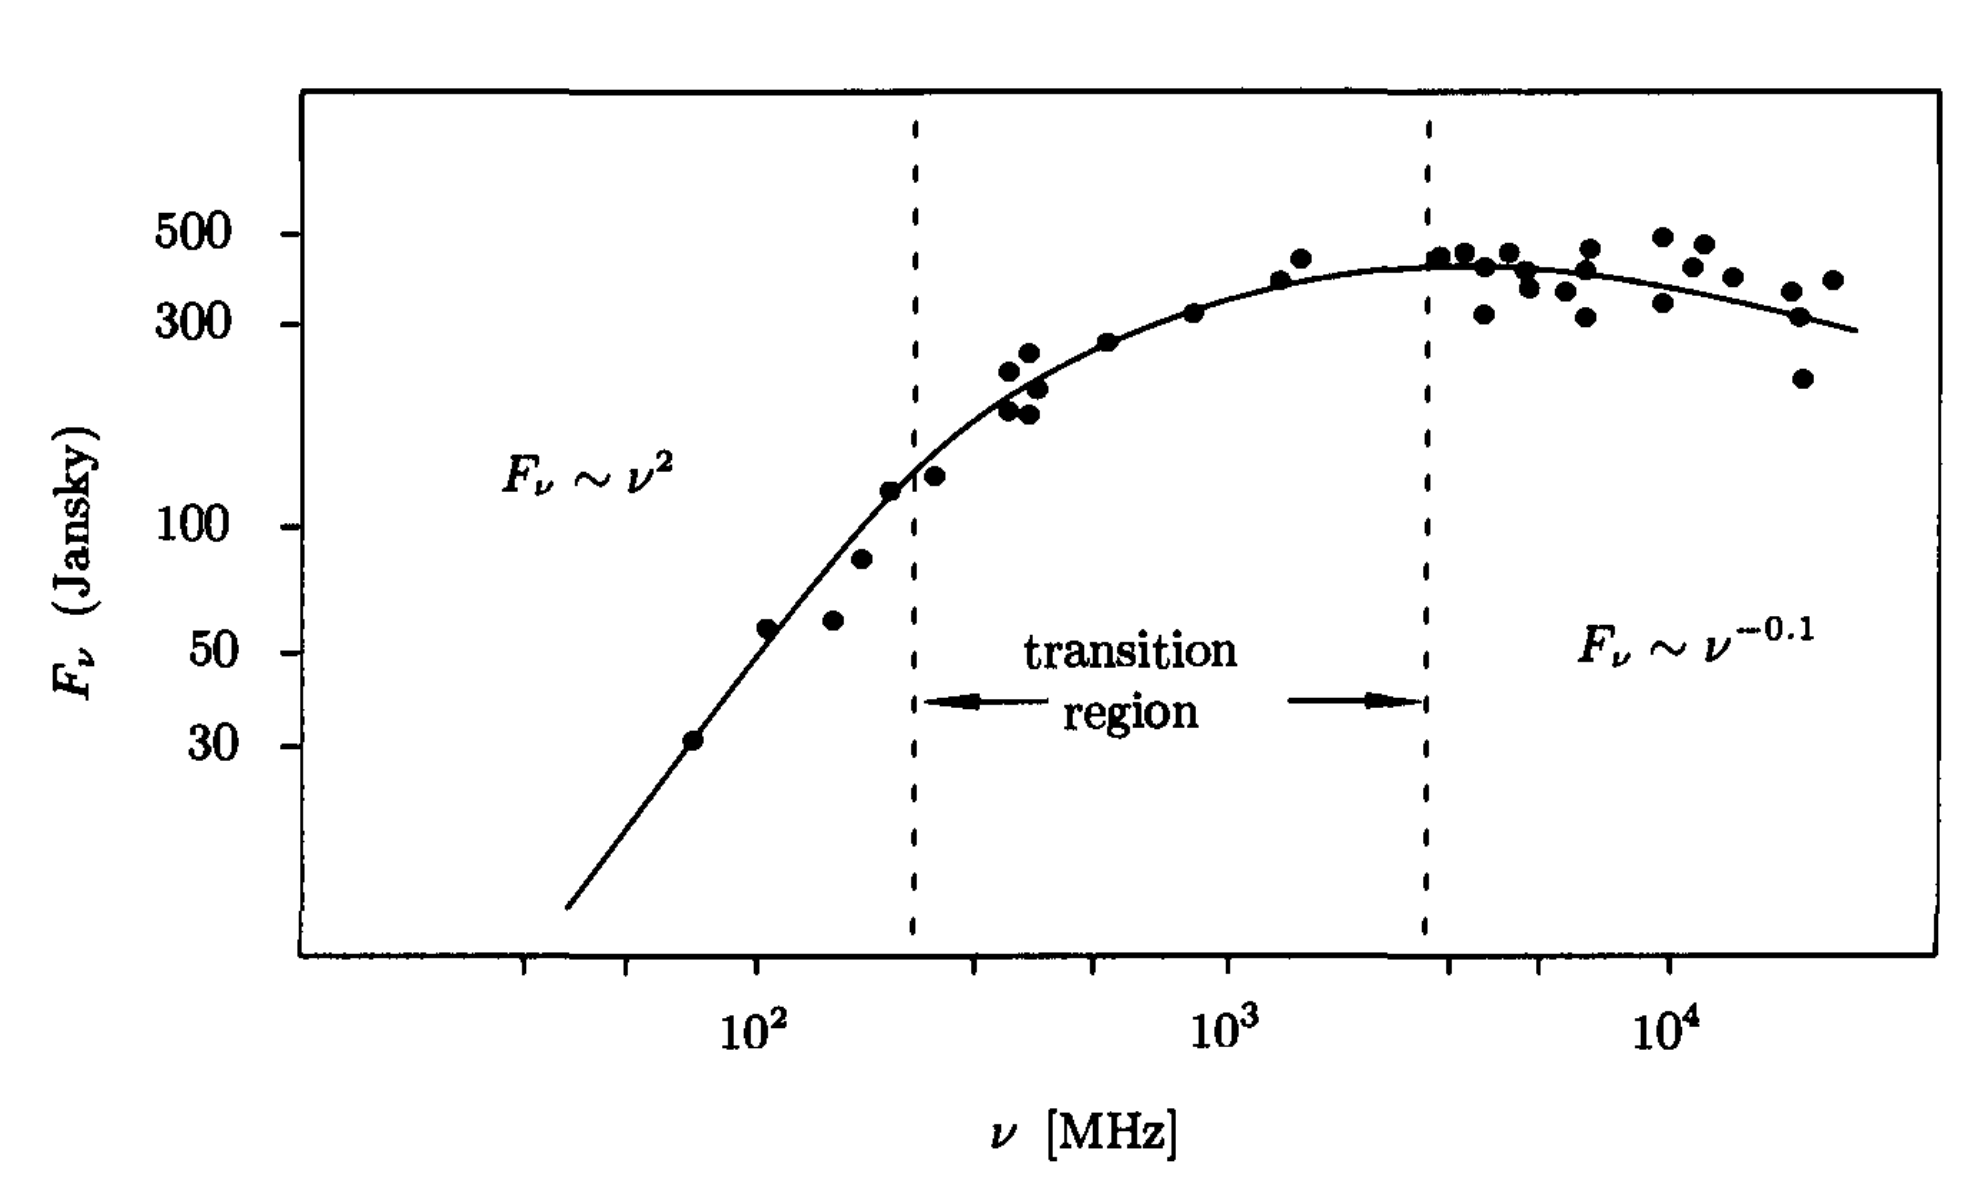
\includegraphics[width=15cm]{FigP4-1.png}
\centering
\caption{(P4.1) Observations of free-free emission from the Orion nebula.}
\end{figure}

Figure 1 (P4.1) contains observations of an $\mathrm{HII}$ region with size $R_S \approx 0.6\,\mathrm{pc}$ in the Orion nebula, which lies at a distance $r \approx 500\,\mathrm{pc}$. Compute approximate values for $T$ and $n_e$ from the data. Quoted values in the literature are $T \approx 8,000 \,{\rm K}$, and $n_e \approx 2,000\,{\rm cm}^{-3}$. Check to see at what frequency $\tau_\nu =1$ for your results. Your derived temperature will not agree with the value $8,000\, {\rm K}$, because the low-frequency measurements have lager effective beam sizes than the high-frequency measurements; thus corrections need to be applied to obtain the true underlying $\nu^2$ dependence at low $\nu$ (see the discussion in Osterbrock 1989, pp. 128-130). This fact should provide a warning against the naive use of free-free radiation to deduce the electron temperature of $\mathrm{HII}$ regions, and partially explains why radio astronomers prefer to use recombination lined for this purpose. 

% --------------------------------------------------------------
%               Solution
% --------------------------------------------------------------

\subsection*{Solution}

To determine the gas temperature, we can use the solutions of $F_\nu$ that were derived above by solving for $T$ then use this to determine $n_e$. Recall our derived solutions for $F_\nu$:

\begin{equation*}
F_\nu =
\left\{
\begin{aligned}
\frac{2\pi k_B}{c^2} \left(\frac{R_S}{r}\right)^2 \nu^2T,       ~~~~~& \mathrm{if}\,\tau_\nu \gg 1 \,\mathrm{(low\,\nu)} \\
(\mathrm{EM})C \frac{2\pi k_B}{c^2} \left(\frac{R_S}{r}\right)^2 \bar{g}_\nu^{ff} T^{-1/2},~~~~~& \mathrm{if}\,\tau_\nu \ll 1 \,\mathrm{(high\,\nu)}
\end{aligned}
\right.
.
\end{equation*}

{\noindent}Using the graph at low radio frequencies, we see that $F_\nu(\nu=10^2\,\mathrm{MHz}) = 50\,\mathrm{Jy}$. Using this to estimate $T$:

\begin{equation*}
\begin{split}
    T &= \frac{c^2}{2\pi k_B} \left(\frac{r}{R_S}\right)^2F_\nu\nu^{-2} \\
    T &= \frac{(2.998\times10^8\mathrm{ms^{-1}})^2}{2\pi (1.38\times10^{-23}\mathrm{m^2\,kg\,s^{-2}\,K^{-1}})} \left(\frac{500\,\mathrm{pc}}{0.6\,\mathrm{pc}}\right)^2(50\,\mathrm{Jy})(10^2\,\mathrm{Hz})^{-2} \\
    T = 35973.77\,\mathrm{K}.
\end{split}
\end{equation*}

{\noindent}This gives us a temperature of

\begin{align*}
    \boxed{T = 35973.77\,\mathrm{K}}.
\end{align*}

{\noindent}We can now use this temperature along with the properties at high radio frequencies to determine $n_e$ using $F_\nu$ at high frequencies:

\begin{equation*}
\begin{split}
    F_\nu = (\mathrm{EM})C \frac{2\pi k_B}{c^2} \left(\frac{R_S}{r}\right)^2 \bar{g}_\nu^{ff} T^{-1/2}.
\end{split}
\end{equation*}

{\noindent}Recalling the definition of the Gaunt factor:

\begin{equation*}
\begin{split}
\bar{g}_\nu^{ff} = \frac{\sqrt3}{2\pi}\left[\ln\left(\frac{8k^3T^3}{\pi^2e^4m_e\nu^2}\right)-5\gamma\right] 
\end{split}
\end{equation*}

{\noindent}and computing its value for our derived temperature $T = 35973.77\,\mathrm{K}$ at a high radio frequency of $10^4\,\mathrm{MHz}$ for which we can read off the graph:

\begin{equation*}
\begin{split}
\bar{g}_\nu^{ff} &= \frac{\sqrt3}{2\pi}\left[\ln\left(\frac{8k_B^3T^3}{\pi^2e^4m_e\nu^2}\right)-5\gamma\right] \\
\bar{g}_\nu^{ff} &= \frac{\sqrt3}{2\pi}\left[\ln\left(\frac{8k_B^3(35973.77\,\mathrm{K})^3}{\pi^2e^4m_e(10^{10}\,\mathrm{Hz})^2}\right)-5(0.5772)\right] \\
\bar{g}_\nu^{ff} &= 5.75.
\end{split}
\end{equation*}

{\noindent}We now compute the constant coefficient:

\begin{equation*}
\begin{split}
C &\equiv \left(\frac{2m_e}{3\pi k_B}\right)^{1/2}\left[\frac{4\pi e^6}{3m_e^2 c k_B}\right] \\
C &= \left[\frac{2(9.109\times10^{-31}\,\mathrm{kg})}{3\pi (1.38\times10^{-23}\,\mathrm{J\,K^{-1}})}\right]^{1/2}\left[\frac{4\pi (1.602\times10^{-19}\,\mathrm{C})^6}{3(9.109\times10^{-31}\,\mathrm{kg})^2 (2.998\times10^8\,\mathrm{m\,s^{-1}}) (1.38\times10^{-23}\,\mathrm{J\,K^{-1}})}\right] \\
C &= 0.0177\,\mathrm{cm^5\,K^{3/2}\,s^{-2}}.
\end{split}
\end{equation*}

{\noindent}Using the graph at low radio frequencies, we see that $F_\nu(\nu=10^4\,\mathrm{MHz}) = 350\,\mathrm{Jy}$. We can now use this and rearrange the $F_\nu$ equation to solve for the emission measure:

\begin{equation*}
\begin{split}
F_\nu &= (\mathrm{EM})C \frac{2\pi k_B}{c^2} \left(\frac{R_S}{r}\right)^2 \bar{g}_\nu^{ff} T^{-1/2} \\
\mathrm{EM} &= F_\nu C^{-1} \frac{c^2}{2\pi k_B} \left(\frac{r}{R_S}\right)^2 (\bar{g}_\nu^{ff})^{-1} T^{1/2} \\
\mathrm{EM} &= (350\,\mathrm{Jy}) (0.0177\,\mathrm{cm^5\,K^{3/2}\,s^{-2}})^{-1} \frac{(2.998\times10^8\,\mathrm{m\,s^{-1}})^2}{2\pi (1.38\times10^{-23}\,\mathrm{J\,K^{-1}})} \left(\frac{500\,\mathrm{pc}}{0.6\,\mathrm{pc}}\right)^2 (5.75)^{-1} (35973.77\,\mathrm{K})^{1/2} \\
\mathrm{EM} &= 4.69\times10^{24}\,\mathrm{cm^{-5}}.
\end{split}
\end{equation*}

{\noindent}Recalling the definition of emission measure, we can now solve for $n_e$ assuming a constant electron density:

\begin{equation*}
\begin{split}
\mathrm{EM} &\equiv \int n_e^2 ds \\
\mathrm{EM} &= n_e^2 \int_0^{2R_S} ds \\
\mathrm{EM} &= n_e^2 (2R_S) \\
n_e &= \sqrt{\frac{\mathrm{EM}}{2R_S}} \\
n_e &= \sqrt{\frac{\mathrm{(4.69\,\mathrm{cm^{-5}})}}{2(0.6\,\mathrm{pc})}} \\
n_e &= 1125.13\,\mathrm{cm^{-3}}.
\end{split}
\end{equation*}

{\noindent}We now have solved for the electron density,

\begin{align*}
    \boxed{n_e = 1125.13\,\mathrm{cm^{-3}}}.
\end{align*}

{\noindent}Lastly, to determine the frequency at which $\tau_\nu = 1$, we simply rearrange the equation for $\tau_\nu$ and solve for $\nu$:


\begin{equation*}
\begin{split}
\tau_\nu &= \mathrm{(EM)} C T^{-3/2} \nu^{-2}\bar{g}_\nu^{ff}(\nu) \\
\nu &= \sqrt{\mathrm{(EM)} C T^{-3/2} (\bar{g}_\nu^{ff})} \\
\nu &= \sqrt{\mathrm{(4.69\times10^{24}\,\mathrm{cm^{-5}})} (0.0177\,\mathrm{cm^5\,K^{3/2}\,s^{-2}}) (35973.77\,\mathrm{K})^{-3/2} (5.75)} \\ 
\nu &= 264.42 \,\mathrm{MHz}.
\end{split}
\end{equation*}

{\noindent}Therefore, the frequency at which $\tau_\nu=1$ is

\begin{align*}
    \boxed{\nu(\tau_\nu = 1) = 264.42 \,\mathrm{MHz}}.
\end{align*}

% --------------------------------------------------------------
%    2. Synchrotron Emission (courtesy of Christopher Pfrommer)
% --------------------------------------------------------------

\section{Synchrotron Emission (courtesy of Christopher Pfrommer)}


% --------------------------------------------------------------
%               Part 1)
% --------------------------------------------------------------

\subsection*{Part 1}

A particle of mass $m$, charge $e$, moves in a plane perpendicular to a uniform, static magnetic field. Work out the total energy emitted per unit time, expressing it in terms of Thomson cross section $\sigma_T$ and magnetic field energy density $U_B = B^2/8\pi$.

% --------------------------------------------------------------
%               Solution
% --------------------------------------------------------------

\subsection*{Solution}

The total radiated power of non-relativistic cyclotron emission with charge $e$ and acceleration $a$ is given by

\begin{align*}
    P_\mathrm{cyc} = \frac{2e^2a^2}{3c^3}.
\end{align*}

{\noindent}For the same charge undergoing relativistic motion, a correction factor of $\gamma^4$ is used for synchrotron emission:

\begin{align*}
    P_\mathrm{syn} = \gamma^4 \frac{2e^2a^2}{3c^3},
\end{align*}

{\noindent}where $\gamma$ is the Lorentz factor 

\begin{align*}
    \gamma \equiv \frac{1}{\sqrt{1 - \frac{v^2}{c^2}}} = \frac{1}{\sqrt{1 - \beta^2}}.
\end{align*}

The equations of motion for a particle of charge $e$ moving relativistically in a magnetic field $\vec{B}$ are

\begin{align*}
    \frac{d}{dt}(\gamma m\vec{v}) = \frac{e}{c} \vec{v} \times \vec{B} \\
    \frac{d}{dt}(\gamma mc^2) = q\vec{v}\cdot\vec{E} = 0.
\end{align*}

{\noindent}Using the first of these, we can solve for the acceleration of motion of a particle moving perpendicular to a uniform, static magnetic field:

\begin{equation*}
\begin{split}
    \frac{d}{dt}(\gamma m\vec{v}) &= \frac{e}{c} \vec{v} \times \vec{B} \\
    \gamma m \frac{d}{dt}(\vec{v}) &= \frac{e}{c} \vec{v} B \\
    \gamma m \vec{a} &= \frac{e}{c} \vec{v} B \\
    \vec{a} &= \frac{eB}{\gamma mc} \vec{v}.
\end{split}
\end{equation*}

{\noindent}Substituting this into our equation for the total radiated power:

\begin{equation*}
\begin{split}
    P_\mathrm{syn} &= \gamma^4 \frac{2e^2a^2}{3c^3} \\
    P_\mathrm{syn} &= \gamma^4 \frac{2e^2}{3c^3} \left(\frac{evB}{\gamma mc}\right)^2 \\
    P_\mathrm{syn} &= \gamma^4 \frac{2e^2}{3c^3} \left(\frac{e^2v^2B^2}{\gamma^2 m^2c^2}\right) \\
    P_\mathrm{syn} &= \gamma^2 \frac{2e^4B^2v^2}{3m^2c^5}.
\end{split}
\end{equation*}

The Thomson scattering cross section $\sigma_T$ is given by

\begin{align*}
    \sigma_T = \frac{8\pi r_0^2}{3},
\end{align*}

{\noindent}where $r_0$ is the ``size'' of the particle given by 

\begin{align*}
    r_0 = \frac{e^2}{mc^2}.
\end{align*}

{\noindent}This allows the Thomson cross section to take the form

\begin{equation*}
\begin{split}
    \sigma_T &= \frac{8\pi r_0^2}{3} \\
    \sigma_T &= \frac{8\pi}{3} \left(\frac{e^2}{mc^2}\right)^2 \\
    \sigma_T &= \left(\frac{8\pi e^4}{3m^2c^4}\right).
\end{split}
\end{equation*}

Re-writing our expression for the total radiated power so that it can be expressed in terms of the Thomson cross section,

\begin{equation*}
\begin{split}
    P_\mathrm{syn} &= \gamma^2 \frac{2e^4B^2v^2}{3m^2c^5} \\
    P_\mathrm{syn} &= 2\gamma^2 B^2v^2 \left(\frac{e^4}{3m^2c^5}\right) \\
    P_\mathrm{syn} &= 2\gamma^2 B^2v^2 \left(\frac{1}{8\pi}\right) \left(\frac{1}{c}\right) \left(\frac{8\pi e^4}{3m^2c^4}\right) \\
    P_\mathrm{syn} &= \frac{\cancel{2}\gamma^2 B^2v^2}{\cancel{8}4\pi c} \left(\frac{8\pi e^4}{3m^2c^4}\right) \\
    P_\mathrm{syn} &= \frac{\gamma^2 B^2v^2}{4\pi c} \sigma_T.
\end{split}
\end{equation*}

The magnetic field energy density is given by 

\begin{align*}
    U_B = \frac{B^2}{8\pi}
\end{align*}

{\noindent}so once more the total radiated power will be re-arranged to be re-written in terms of $U_B$,

\begin{equation*}
\begin{split}
    P_\mathrm{syn} &= \frac{\gamma^2 B^2v^2}{4\pi c} \sigma_T \\
    P_\mathrm{syn} &= \frac{\gamma^2 v^2\sigma_T}{c} \left(\frac{B^2}{4\pi c}\right) \\
    P_\mathrm{syn} &= 2\gamma^2\sigma_T \frac{v^2}{c} \left(\frac{B^2}{8\pi c}\right) \\
    P_\mathrm{syn} &= 2\gamma^2 \frac{v^2}{c} \sigma_T U_B.
\end{split}
\end{equation*}

{\noindent}Since synchrotron radiation is emitted by relativistic electrons, we can take the approximation that $v \approx c$ to simplify the total power:

\begin{align*}
    \boxed{P_\mathrm{syn} = 2\gamma^2 c\sigma_T U_B}.
\end{align*}

% --------------------------------------------------------------
%               Part 2)
% --------------------------------------------------------------

\subsection*{Part 2}

For a tangled magnetic field, this emitted radiation has to be averaged over an isotropic distribution of pitch angles. Let $\alpha$ denote the pitch angle between field and velocity. Take the ultra-relativistic limit and express the total emitted energy in terms of $\gamma = (1 - \beta^2)^{-1/2}$.

% --------------------------------------------------------------
%               Solution
% --------------------------------------------------------------

\subsection*{Solution}

Using the same equation as before to obtain the acceleration while allowing for a pitch angle $\alpha$ between the particle's motion and the magnetic field,

\begin{equation*}
\begin{split}
    \frac{d}{dt}(\gamma m\vec{v}) &= \frac{e}{c} \vec{v} \times \vec{B} \\
    \gamma m \frac{d}{dt}(\vec{v}) &= \frac{e}{c} \vec{v} B \sin\alpha \\
    \gamma m \vec{a} &= \frac{e}{c} \vec{v} B \sin\alpha \\
    \vec{a} &= \frac{eB\sin\alpha}{\gamma mc} \vec{v}.
\end{split}
\end{equation*}

{\noindent}Averaging over all angles, we can obtain the total synchrotron radiated power,

\begin{equation*}
\begin{split}
    P_\mathrm{syn} &= \frac{1}{2\pi}\int_0^{2\pi} \gamma^4 \frac{2e^2}{3c^3}a^2 \\
    P_\mathrm{syn} &= \frac{1}{2\pi}\int_0^{2\pi} \gamma^4 \frac{2e^2}{3c^3} \left(\frac{evB\sin\alpha}{\gamma mc}\right)^2 \\
    P_\mathrm{syn} &= \frac{1}{2\pi}\int_0^{2\pi} \gamma^4 \frac{2e^2}{3c^3} \left(\frac{e^2v^2B^2\sin^2\alpha}{\gamma^2 m^2c^2}\right) \\
    P_\mathrm{syn} &= \frac{1}{2\pi}\int_0^{2\pi} \gamma^2 \frac{2}{3} \frac{e^4v^2B^2}{m^2c^5} \sin^2\alpha \\
    P_\mathrm{syn} &= \frac{1}{2\pi} \gamma^2 \frac{2}{3} \frac{e^4v^2B^2}{m^2c^5} \int_0^{2\pi}\sin^2\alpha \\
    P_\mathrm{syn} &= \frac{1}{\cancel{2}\cancel{\pi}} \gamma^2 \frac{\cancel{2}}{3} \frac{e^4v^2B^2}{m^2c^5} (\cancel{\pi}) \\
    P_\mathrm{syn} &= \gamma^2 \frac{e^4v^2B^2}{3m^2c^5}.
\end{split}
\end{equation*}

{\noindent}Once again, taking the approximation that $v \approx$, this gives us the relativistic synchrotron power for a tangled magnetic field:

\begin{align*}
    \boxed{P_\mathrm{syn} = \gamma^2 \frac{e^4B^2}{3m^2c^3}}.
\end{align*}

% --------------------------------------------------------------
%               Part 3)
% --------------------------------------------------------------

\subsection*{Part 3}

Calculate the time it takes a particle to loose an energy $\Delta E = (\gamma_0 - \gamma)mc^2$ due to synchrotron radiation. How is this expression changed if there are other radiation fields present, e.g., the CMB relic radiation field?

% --------------------------------------------------------------
%               Solution
% --------------------------------------------------------------

\subsection*{Solution}

The cooling time is simply given by the energy divided by the power radiated:

\begin{equation*}
\begin{split}
    t_\mathrm{cool} &\equiv \frac{\Delta E}{P_\mathrm{syn}} \\
    t_\mathrm{cool} &= \frac{(\gamma_0 - \gamma)mc^2}{\left(\gamma^2 \frac{e^4B^2}{3m^2c^3}\right)} \\
    t_\mathrm{cool} &= \frac{(\gamma_0 - \gamma)}{\gamma^2} mc^2 \left(\frac{3m^2c^3}{e^4B^2}\right) \\
    t_\mathrm{cool} &= \frac{(\gamma_0 - \gamma)}{\gamma^2} \left(\frac{3m^3c^5}{e^4B^2}\right).
\end{split}
\end{equation*}

{\noindent}The synchrotron cooling time is therefore

\begin{align*}
    \boxed{t_\mathrm{cool} = \frac{(\gamma_0 - \gamma)}{\gamma^2} \left(\frac{3m^3c^5}{e^4B^2}\right)}.
\end{align*}

{\noindent}If there were other radiation fields present, the power would have to increase resulting in a decreased cooling time.

% --------------------------------------------------------------
%               Part 4)
% --------------------------------------------------------------

\subsection*{Part 4}

Why can proton synchrotron radiation be ignored compared to electron synchrotron? Where
does the mass dependence you find physically arise?

% --------------------------------------------------------------
%               Solution
% --------------------------------------------------------------

\subsection*{Solution}

We can ignore proton synchrotron radiation because the proton mass is very large compared to the electron mass. We can see that the synchrotron radiation power is directly proportional to the acceleration of the charge squared. Since the proton mass is approximately 1,800 times more massive, it will have a significantly reduced acceleration and a resulting synchrotron power that is substantially weaker. Thus, the mass dependence physically arises from the charge's ability to accelerate and thus radiate energy.

% --------------------------------------------------------------
%         3. Intergalactic magnetic field
% --------------------------------------------------------------

\section{Intergalactic magnetic field}

Synchrotron radiation at sub-GHz radio frequencies is currently the most sensitive direct way to trace widespread intergalactic magnetic fields down to about $0.1\,\mu\mathrm{G}$. The first successful attempt to detect the presence of such a field is at $326\,\mathrm{MHz}$ (Kim, Kronberg, Giovannini \& Venturi, 1989, Nature 341, 720, the first two authors were from Toronto).

% --------------------------------------------------------------
%               Part 1)
% --------------------------------------------------------------

\subsection*{Part 1}

To obtain a magnetic field strength using the observed flux, it is common to adopt an assumption called `minimum energy' assumption (thus the associated `minimum energy field'). Assume cosmic ray electrons have a single $\gamma$ factor but isotropic pitch angles (see last question). Write down the sum of the electron kinetic energy and magnetic field energy. For a given synchrotron luminosity, this sum reaches a minimum at $B = B_\mathrm{min}$. Determine $B_\mathrm{min}$. How different is this field strength from `equipartition field'?

% --------------------------------------------------------------
%               Solution
% --------------------------------------------------------------

\subsection*{Solution}

The kinetic energy of relativistic electrons is given by

\begin{align*}
    E_K \approx \gamma n_e m_ec^2
\end{align*}

{\noindent}while the magnetic energy density is given by

\begin{align*}
    U_B = \frac{B^2}{8\pi}.
\end{align*}

{\noindent}Thus, the sum of electron kinetic and magnetic field energy is:

\begin{align*}
    \boxed{E_\mathrm{tot} = \gamma n_e m_ec^2 + \frac{B^2}{8\pi}}.
\end{align*}

{\noindent}Recall that the synchrotron frequency $\nu_\mathrm{sync}$ is given by

\begin{align*}
    \nu_\mathrm{sync} = \gamma^2 \frac{eB}{m_ec},
\end{align*}

{\noindent}which can be rearranged to express $\gamma$ in terms of properties of synchrotron radiation:

\begin{align*}
    \gamma = \sqrt{\nu_\mathrm{sync} \frac{m_ec}{eB}}.
\end{align*}

{\noindent}Plugging this expression for $\gamma$ into $E_\mathrm{tot}$:

\begin{equation*}
\begin{split}
    E_\mathrm{tot} &= \gamma n_e m_ec^2 + \frac{B^2}{8\pi} \\
    E_\mathrm{tot} &= \left(\sqrt{\nu_\mathrm{sync} \frac{m_ec}{eB}}\right) n_e m_ec^2 + \frac{B^2}{8\pi}.
\end{split}
\end{equation*}

{\noindent}Now we can find the minimum energy $B_\mathrm{min}$ by calculating $dE_\mathrm{tot}/dB = 0$ and solving for $B_\mathrm{min}$:

\begin{equation*}
\begin{split}
    0 &= \frac{d}{dB}E_\mathrm{tot} = \frac{d}{dB} \left( \sqrt{\nu_\mathrm{sync} \frac{m_ec}{eB}} n_e m_ec^2 + \frac{B^2}{8\pi} \right) \\
    0 &= \frac{d}{dB} \left( \sqrt{\nu_\mathrm{sync} \frac{m_ec}{eB}} n_e m_ec^2 \right) + \frac{d}{dB} \left( \frac{B^2}{8\pi} \right) \\
    0 &= n_e m_ec^2 \sqrt{\nu_\mathrm{sync} \frac{m_ec}{e}} \frac{d}{dB} \left( B^{-1/2} \right) + \frac{1}{8\pi}\frac{d}{dB} \left( B^2 \right) \\
    0 &= n_e m_ec^2 \sqrt{\nu_\mathrm{sync} \frac{m_ec}{e}} \left( \frac{-1}{2}B^{-3/2} \right) + \frac{1}{\cancel{8}4\pi}\left( \cancel{2}B \right) \\
    \frac{B}{4\pi} &= n_e m_ec^2 \sqrt{\nu_\mathrm{sync} \frac{m_ec}{e}} \left( \frac{1}{2}B^{-3/2} \right) \\
    B^{3/2}B &= \cancel{4}2\pi\frac{n_e m_ec^2}{\cancel{2}} \sqrt{\nu_\mathrm{sync} \frac{m_ec}{e}} \\
    B^{5/2} &= 2\pi n_e m_ec^2 \sqrt{\nu_\mathrm{sync} \frac{m_ec}{e}} \\
    B &= \left(2\pi n_e m_ec^2\sqrt{\nu_\mathrm{sync}\frac{m_ec}{e}} \right)^{2/5} \\
    B &= \left(2\pi n_em_ec^2\right)^{2/5} \left(\nu_\mathrm{sync}\frac{m_ec}{e}\right)^{1/5} \\
    B &= \left(2\pi n_e\right)^{2/5} m_e^{2/5}c^{4/5} \left(\frac{\nu_\mathrm{sync}}{e}\right)^{1/5} m_e^{1/5}c^{1/5} \\
    B &= \left(2\pi n_e\right)^{2/5} m_e^{3/5}c \left(\frac{\nu_\mathrm{sync}}{e}\right)^{1/5} \\
    B &= \left(2^2\pi^2 n_e^2 m_e^3 \frac{\nu_\mathrm{sync}}{e}\right)^{1/5} c \\
    B &= \left(\frac{\nu_\mathrm{sync}4\pi^2 n_e^2 m_e^3}{e}\right)^{1/5} c.
\end{split}
\end{equation*}

{\noindent}Thus we see that the minimum energy $B$ is given by:

\begin{align*}
    \boxed{B = \left(\frac{\nu_\mathrm{sync}4\pi^2 n_e^2 m_e^3}{e}\right)^{1/5} c}.
\end{align*}

This is different from an `equipartition field' because we did not assume $E_K = U_B$.

% --------------------------------------------------------------
%               Part 2)
% --------------------------------------------------------------

\subsection*{Part 2}

A somewhat more complicated derivation is given in P. 179 of Shu where he accounts for a power-law distribution of electrons. We will adopt his results here. The measured flux at $326\,\mathrm{MHz}$ is $760\,\mathrm{mJ}y$, while at $430\,\mathrm{MHz}$ is $600\,\mathrm{mJy}$. This is roughly consistent with a spectral index $\alpha_\nu = 1.5$ where $F_\nu \propto \nu^{-\alpha_\nu}$. Follow the authors in assuming a geometry for the radiating region: a $1900\,\mathrm{kpc}$ long of cylinder with $800\,\mathrm{kps}$ in diameter. What do you obtain for the minimum energy field?

% --------------------------------------------------------------
%               Solution
% --------------------------------------------------------------

\subsection*{Solution}

Using the results of Shu for the equipartition field, we see that:

\begin{align*}
    U_{CR} = \frac{4}{p+1}U_B, ~~~~~~~~~~ U_{CR} = \frac{n_0m_ec^2}{2-p}\gamma_\mathrm{min}^{(2-p)}.
\end{align*}

{\noindent}Equating these two expressions for $U_\mathrm{CR}$ allows us to solve for $U_B$:

\begin{align*}
    \frac{4}{p+1}U_B &= \frac{n_0m_ec^2}{2-p}\gamma_\mathrm{min}^{(2-p)} \\
    U_B &= \left(\frac{p+1}{4}\right)\frac{n_0m_ec^2}{2-p}\gamma_\mathrm{min}^{(2-p)}.
\end{align*}

{\noindent}Following Shu, we can choose $\gamma_\mathrm{min}$ such that $\gamma_\mathrm{min}^2\nu_L$ gives us the lowest frequency for synchrotron radiation. This gives us an expression for $\nu_\mathrm{obs}$ which can be rearranged to solve for $\gamma_\mathrm{min}$:

\begin{align*}
    \nu_\mathrm{obs} = \gamma_\mathrm{min}^2 \frac{eB}{2\pi m_ec} \\
    \gamma_\mathrm{min} = \sqrt{\frac{\nu_\mathrm{obs}}{\frac{eB}{2\pi m_ec}}} \\
    \gamma_\mathrm{min} = \sqrt{{\frac{2\pi m_ec\nu_\mathrm{obs}}{eB}}}.
\end{align*}

{\noindent}Once again following Shu, we can use the following equations to determine $n_0$:

\begin{align*}
    \rho j_\nu \sim \frac{2}{3}c\sigma_Tn_0U_B\nu_L^{-1}\left(\frac{\nu}{\nu_L}\right)^{(1-p)/2}, ~~~~~~~~~~ L_\nu = \int_V \rho j_\nu dV = \rho j_\nu V.
\end{align*}

{\noindent}Plugging the expression for $\rho j_\nu$ into $L_\nu$ and rearranging for $n_0$:

\begin{align*}
    L_\nu = \left(\frac{2}{3}c\sigma_Tn_0U_B\nu_L^{-1}\left(\frac{\nu}{\nu_L}\right)^{(1-p)/2}\right) V \\
    n_0 = \frac{3}{2}c^{-1}\sigma_T^{-1}U_B^{-1}\nu_L\left(\frac{\nu}{\nu_L}\right)^{(p-1)/2} V^{-1} L_\nu \\
    n_0 = \frac{3\nu^{(p-1)/2}L_\nu}{2c\sigma_TU_BV} \nu_L \nu_L^{(1-p)/2} \\
    n_0 = \frac{3\nu^{(p-1)/2}\nu_L^{(3-p)/2}L_\nu}{2c\sigma_TU_BV} \\
    n_0 = \frac{3\nu^{(p-1)/2}\nu_L^{(3-p)/2}L_\nu}{2c\sigma_T(B^2/8\pi)V} \\
    n_0 = \frac{(\cancel{8}4\pi)3\nu^{(p-1)/2}\nu_L^{(3-p)/2}L_\nu}{\cancel{2}c\sigma_T(B^2)V} \\
    n_0 = \frac{12\pi\nu^{(p-1)/2}\nu_L^{(3-p)/2}L_\nu}{c\sigma_T(B^2)V}.
\end{align*}

{\noindent}Plugging these into our equation for $U_B$ and noting that $U_B = B^2/8\pi$, we can now solve for $B$:

\begin{align*}
    \frac{B^2}{8\pi} &= \left(\frac{p+1}{4}\right)\frac{n_0m_ec^2}{2-p}\gamma_\mathrm{min}^{(2-p)} \\
    \frac{B^2}{8\pi} &= \left(\frac{p+1}{4}\right)\frac{\left( \frac{12\pi\nu^{(p-1)/2}\nu_L^{(3-p)/2}L_\nu}{c\sigma_T(B^2)V} \right) m_ec^2}{2-p} \left( \sqrt{{\frac{2\pi m_ec\nu_\mathrm{obs}}{eB}}} \right)^{(2-p)} \\
    \frac{B^2}{8\pi} &= \left(\frac{p+1}{\cancel{4}}\right) \left( \frac{\cancel{12}3\pi\nu^{(p-1)/2}\nu_L^{(3-p)/2}L_\nu}{c\sigma_T(B^2)V(2-p)} \right) m_ec^2 \left({\frac{2\pi m_ec\nu_\mathrm{obs}}{eB}} \right)^{(2-p)/2} \\
    \frac{B^2}{8\pi} &= (p+1) \left( \frac{3\pi\nu^{(p-1)/2}\nu_L^{(3-p)/2}L_\nu}{c\sigma_TV(2-p)} \right) \left(B^{-2}\right) m_ec^2 \left({\frac{2\pi m_ec\nu_\mathrm{obs}}{e}} \right)^{(2-p)/2} \left(B^{(p-2)/2}\right) \\
    \left(B^4\right) \left(B^{(2-p)/2}\right) &= 8\pi (p+1) \left( \frac{3\pi\nu^{(p-1)/2}\nu_L^{(3-p)/2}m_ec^2L_\nu}{c\sigma_TV(2-p)} \right) \left({\frac{2\pi m_ec\nu_\mathrm{obs}}{e}} \right)^{(2-p)/2} \\
    B^{(10-p)/2} &= 8\pi (p+1) \nu_L^{(3-p)/2} \left( \frac{3\pi\nu^{(p-1)/2}m_ec^2L_\nu}{c\sigma_TV(2-p)} \right) \left({\frac{2\pi m_ec\nu_\mathrm{obs}}{e}} \right)^{(2-p)/2} \\
    B^{(10-p)/2} &= 8\pi (p+1) \left(\frac{eB}{2\pi m_e}\right)^{(3-p)/2} \left( \frac{3\pi\nu^{(p-1)/2}m_ec^2L_\nu}{c\sigma_TV(2-p)} \right) \left({\frac{2\pi m_ec\nu_\mathrm{obs}}{e}} \right)^{(2-p)/2} \\
    B^{(10-p)/2} &= 8\pi (p+1) \left(\frac{e}{2\pi m_e}\right)^{(3-p)/2} B^{(3-p)/2} \left( \frac{3\pi\nu^{(p-1)/2}m_ec^2L_\nu}{c\sigma_TV(2-p)} \right) \left({\frac{2\pi m_ec\nu_\mathrm{obs}}{e}} \right)^{(2-p)/2}
\end{align*}

\begin{align*}
    B^5B^{-p/2}B^{(p-3)/2} &= 8\pi (p+1) \left(\frac{e}{2\pi m_e}\right)^{(3-p)/2} \left( \frac{3\pi\nu^{(p-1)/2}m_ec^2L_\nu}{c\sigma_TV(2-p)} \right) \left({\frac{2\pi m_ec\nu_\mathrm{obs}}{e}} \right)^{(2-p)/2} \\
    B^{7/2} &= 8\pi (p+1) \left(\frac{e}{2\pi m_e}\right)^{(3-p)/2} \left( \frac{3\pi\nu^{(p-1)/2}m_ec^2L_\nu}{c\sigma_TV(2-p)} \right) \left({\frac{2\pi m_ec\nu_\mathrm{obs}}{e}} \right)^{(2-p)/2} \\
    B &= 8^{2/7}\pi^{2/7} (p+1)^{2/7} \left(\frac{e}{2\pi m_e}\right)^{(3-p)/7} \left( \frac{3\pi\nu^{(p-1)/2}m_ec^2L_\nu}{c\sigma_TV(2-p)} \right)^{2/7} \left({\frac{2\pi m_ec\nu_\mathrm{obs}}{e}} \right)^{(2-p)/7} \\
    B &= 8^{2/7}\pi^{2/7} \left(\frac{p+1}{2-p}\right)^{2/7} \left(\frac{e}{2\pi m_e}\right)^{(3-p)/7} \left( \frac{3\pi\nu^{(p-1)/2}m_ec^2L_\nu}{c\sigma_TV} \right)^{2/7} \left({\frac{2\pi m_ec\nu_\mathrm{obs}}{e}} \right)^{(2-p)/7} \\
    B &= \pi^{3/7} \left[\left(\frac{p+1}{2-p}\right) \left(\frac{24L_\nu}{\sigma_TV}\right)\right]^{2/7} \left(\frac{em_ec\nu_\mathrm{obs}}{2}\right)^{1/7}.
\end{align*}

{\noindent}Thus our final result for the minimum $B$ field is:

\begin{align*}
    \boxed{B = \pi^{3/7} \left[\left(\frac{p+1}{2-p}\right) \left(\frac{24L_\nu}{\sigma_TV}\right)\right]^{2/7} \left(\frac{em_ec\nu_\mathrm{obs}}{2}\right)^{1/7}}.
\end{align*}

Now, using the result of Shu, we know that the power-law distribution of electrons follows a spectral index of $\alpha_\nu = 1.5$ where $F_\nu \propto \nu^{-\alpha_\nu}$. We can use the following relations to solve for what this means for $p$:

\begin{align*}
    F_\nu \propto \nu^{-\alpha_\nu},~~~~~~~~~~ L_\nu \propto \nu^{(1-p)/2}
\end{align*}

\begin{align*} \rightarrow -\alpha_\nu &= \frac{1-p}{2} \\
    2\alpha_\nu &= p-1 \\
    p &= 2(1.5) + 1 \\
    p &= 4.
\end{align*}

{\noindent}We are now set to calculate the minimum $B$ field:

\begin{align*}
    B &= \pi^{3/7} \left[\left(\frac{5}{\cancel{2}}\right) \left(\frac{\cancel{24}12(4\pi d^2 F_\nu)}{\sigma_TV}\right)\right]^{2/7} \left(\frac{em_ec\nu_\mathrm{obs}}{2}\right)^{1/7} \\
    B &= \pi^{3/7} \left[\frac{240\pi (100\,\mathrm{Mpc})^2 (760\,\mathrm{mJy})}{\sigma_T\pi(400\,\mathrm{kpc})^2(1900\,\mathrm{kpc})}\right]^{2/7} \left(\frac{em_ec(326\,\mathrm{MHz})}{2}\right)^{1/7}  \\
    B &= 2.9 \times 10^{-8}\,\mathrm{kg^{1/2}\,m^{-1/2}s^{-1}},
\end{align*}

{\noindent}where we have used the volume of the cylindrical region as $V = \pi R^2 L$. We can now use this to determine $U_B$:

\begin{align*}
    U_B &= \frac{B^2}{8\pi} \\
    U_B &= \frac{(2.9 \times 10^{-8}\,\mathrm{kg^{1/2}\,m^{-1/2}s^{-1}})^2}{8\pi} \\
    U_B &= 3.4 \times 10^{-17} \,\mathrm{kg\,m^{-1}\,s^{-2}}.
\end{align*}

{\noindent}Therefore, the minimum field energy density is:

\begin{align*}
    \boxed{U_B = 3.4 \times 10^{-17} \,\mathrm{kg\,m^{-1}\,s^{-2}}}.
\end{align*}


% --------------------------------------------------------------
%               Part 3)
% --------------------------------------------------------------

\subsection*{Part 3}

For the electrons responsible for the $326\,\mathrm{MHz}$ radiation, what is their synchrotron cooling time?

% --------------------------------------------------------------
%               Solution
% --------------------------------------------------------------

\subsection*{Solution}



% --------------------------------------------------------------
%               Part 4)
% --------------------------------------------------------------

\subsection*{Part 4}

Inverse-compton scattering of CMB photons can also lead to cooling. Calculate the energy density of a $3\,\mathrm{K}$ background glow. Now what is the inverse-compton cooling time for the same electrons? At what wavelength band should we expect to observe the 'cooling' radiation?

% --------------------------------------------------------------
%               Solution
% --------------------------------------------------------------

\subsection*{Solution}








% --------------------------------------------------------------
%       4. Radio Emission from Normal Galaxies (non-AGN)
% --------------------------------------------------------------

\section{Radio Emission from Normal Galaxies (non-AGN)}

One of the tightest correlation in astronomy is the FIR/radio correlation of normal galaxies (see Fig. 8 of Condon, Annual Review of Astronomy \& Astrophysics, 1992, whereas Fig. 1 shows the the spectral energy distribution for a typical galaxy FIR/radio band). The far infrared luminosities of galaxies scale roughly linearly with their radio luminosities over four orders of magnitude. This is surprising in more than one ways. We will try to appreciate the physics behind this correlation, following the narratives of Condon (1992).

% --------------------------------------------------------------
%               Part 1)
% --------------------------------------------------------------

\subsection*{Part 1}

Far-infrared light from a galaxy can dominate its total energy output. This arises from dust reprocessing of star light, therefore it depends on the dust temperature and the dust size distribution. Assume that grains of size $\sim\,0.05\,\mu\mathrm{m}$ are responsible, that at FIR the galaxy is optically thin, that dust is embedded in a radiation field with energy density of $U_r \sim 10-12\,\mathrm{erg\,cm^{-3}}$ (the Milky Way value) with typical photons in the optical. Obtain the dust temperature and show that most of the dust radiation indeed occurs in FIR ($\sim\,100\,\mu\mathrm{m}$). Then follow the lead of the article to obtain his Eq. 26. This relates LFIR with the current star formation rate.

% --------------------------------------------------------------
%               Solution
% --------------------------------------------------------------

\subsection*{Solution}

Since the FIR luminosity is reprocessed optical starlight being re-emitted in the FIR, we begin by noting that the absorbed power should be equal to the re-emitted power. The absorbed power is given by 

\begin{align*}
    P_\mathrm{abs} &= F_\mathrm{abs}\sigma_\mathrm{abs} \\
    P_\mathrm{abs} &= (U_rc) (Q_\mathrm{abs}\pi s^2) \\
    P_\mathrm{abs} &= U_rc \left(\frac{s}{\lambda_\mathrm{optical}}\right) \pi s^2 \\
    P_\mathrm{abs} &= U_rc \left(\frac{\pi s^3}{\lambda_\mathrm{optical}}\right).
\end{align*}

{\noindent}Similarly, the re-emitted power is given by

\begin{align*}
    P_\mathrm{emit} &= Q_\mathrm{emit} A \sigma_\mathrm{emit} T^4 \\
    P_\mathrm{emit} &= \left(\frac{s}{\lambda_\mathrm{FIR}}\right) (4\pi s^2) \sigma_\mathrm{emit} T^4 \\
    P_\mathrm{emit} &= \left(\frac{4\pi s^3}{\lambda_\mathrm{FIR}}\right) \sigma_\mathrm{emit} T^4.
\end{align*}

{\noindent}Equating the two and solving for the dust temperature:

\begin{align*}
    P_\mathrm{abs} &= P_\mathrm{emit} \\
    U_rc \left(\frac{\pi s^3}{\lambda_\mathrm{optical}}\right) &= \left(\frac{4\pi s^3}{\lambda_\mathrm{FIR}}\right) \sigma_\mathrm{emit} T^4 \\
    U_rc \left(\frac{\pi s^3}{\lambda_\mathrm{optical}}\right) &= \left(\frac{4\pi s^3}{0.0029\,\mathrm{m\,K}/T}\right) \sigma_\mathrm{emit} T^4 \\
    U_rc \left(\frac{\cancel{\pi} \cancel{s^3}}{\lambda_\mathrm{optical}}\right) &= \left(\frac{4\cancel{\pi} \cancel{s^3}}{0.0029\,\mathrm{m\,K}}\right) \sigma_\mathrm{emit} T^5 \\
    T^5 &= U_rc \left(\frac{1}{\lambda_\mathrm{optical}}\right) \left(\frac{0.0029\,\mathrm{m\,K}}{4}\right) \sigma_\mathrm{emit}^{-1} \\
    T &= \left[\frac{(0.000725\,\mathrm{m\,K}) U_rc}{\lambda_\mathrm{optical}\sigma_\mathrm{emit}}\right]^{1/5} \\
    T &= \left[\frac{(0.000725\,\mathrm{m\,K}) (10\,\mathrm{erg\,cm^{-3}})(2.998\times10^8\,\mathrm{m\,s^{-1}})}{(0.5\,\mu\mathrm{m})\sigma_\mathrm{emit}}\right]^{1/5} \\
    T &= 15 \,\mathrm{K}.
\end{align*}

{\noindent}Therefore, the FIR dust temperature must be

\begin{align*}
    \boxed{T = 15 \,\mathrm{K}}.
\end{align*}

{\noindent}To determine the $\lambda_\mathrm{FIR}$,

\begin{align*}
    \lambda_\mathrm{FIR} &= \frac{0.0029\,\mathrm{m\,K}}{T} \\
    \lambda_\mathrm{FIR} &= \frac{0.0029\,\mathrm{m\,K}}{15 \,\mathrm{K}} \\
    \lambda_\mathrm{FIR} &= 0.000193\,\mathrm{m} \\
    \lambda_\mathrm{FIR} &= 193\,\mu\mathrm{m}.
\end{align*}

{\noindent}Thus, the associated wavelength of the FIR dust emission is

\begin{align*}
    \boxed{\lambda_\mathrm{FIR} = 193\,\mu\mathrm{m}},
\end{align*}

{\noindent}which is approximately $100\,\mu\mathrm{m}$ as desired.

% --------------------------------------------------------------
%               Part 2)
% --------------------------------------------------------------

\subsection*{Part 2}

In contrast, the radio luminosity is only some $10^{−4}$ of the bolometric luminosity. However, this luminosity is also related to the star formation rate. Show that the thermal radio luminosity, arising from free-free radiation from electrons in $\mathrm{HII}$ regions around massive stars, is as expressed in his Eq. 2 (you may need to refer to Shu for the relevant Gaunt factor, which roughly scales as $\nu^{-0.1}$). Depending on the values of order-unity coefficients that you adopt, you may find a slightly different expression as Condon does. After this, follow the lead of the article to obtain Eq. 23, where LT (thermal radio luminosity) is also related to the current star formation rate.

% --------------------------------------------------------------
%               Solution
% --------------------------------------------------------------

\subsection*{Solution}

\begin{align*}
    \frac{N_{u\nu}}{S^{-1}} \geq 6.3\times10^{52} \left(\frac{T_e}{10^4\,\mathrm{K}}\right)^{-0.45} \left(\frac{\nu}{\mathrm{GHz}}\right)^{0.1} \left(\frac{L_T}{10^{20}\,\mathrm{W\,Hz^{-1}}}\right)~~~~~[\mathrm{Eq.\,2}]
\end{align*}

\begin{align*}
    \left(\frac{L_T}{10^{20}\,\mathrm{W\,Hz^{-1}}}\right) \sim 5.5\times10^{20} \left(\frac{\nu}{\mathrm{GHz}}\right)^{-0.1} \left[\frac{\mathrm{SFR}(M\geq5\,M_\odot)}{M_\odot\,\mathrm{yr^{-1}}}\right] ~~~~~[\mathrm{Eq.\,23}]
\end{align*}

{\noindent}Equation 3 of Condon gives us the $H\beta$ flux as

\begin{align*}
    \left(\frac{F(H\beta)}{10^{-12}\,\mathrm{erg\,cm^{-2}s^{-1}}}\right) \sim 0.28 \left(\frac{T_e}{10^4\,\mathrm{K}}\right)^{-0.52} \left(\frac{\nu}{\mathrm{GHz}}\right)^{0.1} \left(\frac{S_T}{\mathrm{mJy}}\right),
\end{align*}

{\noindent}which is related to the $H\alpha$ flux in Eq. 4a as

\begin{align*}
    \frac{F(H\alpha)}{F(H\beta)} = 2.86 \left(\frac{T_e}{10^4\,\mathrm{K}}\right)^{-0.07}.
\end{align*}

{\noindent}Noting that the luminosity can be written in terms of the flux as $L_\nu = F_\nu A$ where $A$ is the emitting area, and using the aforementioned expression for $H\beta$ flux, this allows us to write the $H\alpha$ luminosity as

\begin{align*}
    L(H\alpha) &= F(H\alpha) A \\
    L(H\alpha) &= 2.86 \left(\frac{T_e}{10^4\,\mathrm{K}}\right)^{-0.07} F(H\beta) A \\
    L(H\alpha) &= 2.86 \left(\frac{T_e}{10^4\,\mathrm{K}}\right)^{-0.07} \left[ 0.28 \left(\frac{T_e}{10^4\,\mathrm{K}}\right)^{-0.52} \left(\frac{\nu}{\mathrm{GHz}}\right)^{0.1} \left(\frac{S_T}{\mathrm{mJy}}\right) 10^{-12}\mathrm{erg\,cm^{-2}s^{-1}} \right] A \\
    L(H\alpha) &= 0.8 \left(\frac{T_e}{10^4\,\mathrm{K}}\right)^{-0.59} \left(\frac{\nu}{\mathrm{GHz}}\right)^{0.1} \left(\frac{S_T}{10^{-33}\mathrm{W\,cm^{-2}Hz^{-2}}}\right) (10^{-12}\,\mathrm{erg\,cm^{-2}s^{-1}}) A \\
    L(H\alpha) &= 0.8 \left(\frac{T_e}{10^4\,\mathrm{K}}\right)^{-0.59} \left(\frac{\nu}{\mathrm{GHz}}\right)^{0.1} \left(\frac{L_T/\cancel{A}}{10^{-33}\mathrm{\cancel{W}\,\cancel{cm^{-2}}Hz^{-\cancel{2}1}}}\right) (10^{-12}\,\mathrm{10^{-7}\,\cancel{W}\,\cancel{s}\,\cancel{cm^{-2}}\cancel{s^{-1}}}) \cancel{A} \\
    L(H\alpha) &= 0.8 \left(\frac{T_e}{10^4\,\mathrm{K}}\right)^{-0.59} \left(\frac{\nu}{\mathrm{GHz}}\right)^{0.1} \left(\frac{L_T}{10^{-33}\mathrm{Hz^{-1}}}\right) (10^{-19}) \\
    L(H\alpha) &= 0.8\times10^{14} \left(\frac{T_e}{10^4\,\mathrm{K}}\right)^{-0.59} \left(\frac{\nu}{\mathrm{GHz}}\right)^{0.1} \left(\frac{L_T}{\mathrm{Hz^{-1}}}\right).
\end{align*}

{\noindent}Plugging this into Eq. 22 of Condon

\begin{align*}
    \left(\frac{L(H\alpha)}{\mathrm{W}}\right) &\sim 4.4\times10^{34} \left[\frac{\mathrm{SFR}(M \geq 5M_\odot)}{M_\odot\,\mathrm{yr^{-1}}}\right] \\
    0.8\times10^{14} \left(\frac{T_e}{10^4\,\mathrm{K}}\right)^{-0.59} \left(\frac{\nu}{\mathrm{GHz}}\right)^{0.1} \left(\frac{L_T}{\mathrm{W\,Hz^{-1}}}\right) &\sim 4.4\times10^{34} \left[\frac{\mathrm{SFR}(M \geq 5M_\odot)}{M_\odot\,\mathrm{yr^{-1}}}\right] 
\end{align*}

{\noindent}and now solving for the radio thermal luminosity:

\begin{align*}
    \left(\frac{L_T}{\mathrm{W\,Hz^{-1}}}\right) &\sim (0.8\times10^{-14}) 4.4\times10^{34} \left(\frac{\nu}{\mathrm{GHz}}\right)^{-0.1} \left(\frac{T_e}{10^4\,\mathrm{K}}\right)^{0.59} \left[\frac{\mathrm{SFR}(M \geq 5M_\odot)}{M_\odot\,\mathrm{yr^{-1}}}\right] \\
    \left(\frac{L_T}{\mathrm{W\,Hz^{-1}}}\right) &\sim 5.5\times10^{20} \left(\frac{\nu}{\mathrm{GHz}}\right)^{-0.1} \left(\frac{T_e}{10^4\,\mathrm{K}}\right)^{0.59} \left[\frac{\mathrm{SFR}(M \geq 5M_\odot)}{M_\odot\,\mathrm{yr^{-1}}}\right].
\end{align*}

{\noindent}This is Eq. 23 of Codon that we were after:

\begin{align*}
    \boxed{\left(\frac{L_T}{\mathrm{W\,Hz^{-1}}}\right) \sim 5.5\times10^{20} \left(\frac{\nu}{\mathrm{GHz}}\right)^{-0.1} \left(\frac{T_e}{10^4\,\mathrm{K}}\right)^{0.59} \left[\frac{\mathrm{SFR}(M \geq 5M_\odot)}{M_\odot\,\mathrm{yr^{-1}}}\right]}.
\end{align*}


% --------------------------------------------------------------
%               Part 3)
% --------------------------------------------------------------

\subsection*{Part 3}

Obtain the value of $q$ (eq. 15) based on the above LFIR and LT . You should find that while you get the observed linear relationship, the normalization seems off.

% --------------------------------------------------------------
%               Solution
% --------------------------------------------------------------

\subsection*{Solution}

Eq. 15 of Codon provides the definition of the parameter $q$:

\begin{align*}
    q &\equiv \log \left(\frac{\mathrm{FIR}}{3.75\times10^{12}\,\mathrm{W\,m^{-2}}}\right) - \log \left(\frac{S_\nu}{\mathrm{W\,m^{-2}\,Hz^{-1}}}\right) \\
    q &= \log \left(\frac{L_\mathrm{FIR}/A}{3.75\times10^{12}\,\mathrm{W\,m^{-2}}}\right) - \log \left(\frac{L_T/A}{\mathrm{W\,m^{-2}\,Hz^{-1}}}\right) \\
    q &= \log \left(\frac{L_\mathrm{FIR}/\cancel{A}}{3.75\times10^{12}\,\mathrm{\cancel{W}\,\cancel{m^{-2}}}} \frac{\mathrm{\cancel{W}\,\cancel{m^{-2}}\,Hz^{-1}}}{L_T/\cancel{A}} \right) \\
    q &= \log \left(\frac{L_\mathrm{FIR}}{3.75\times10^{12}} \frac{\mathrm{Hz^{-1}}}{L_T} \right) \\
    q &= \log \left( \frac{1.1\times10^{10} \left[\cancel{\frac{\mathrm{SFR}(M\geq 5M_\odot)}{M_\odot \mathrm{yr^{-1}}}}\right]L_\odot \,\mathrm{Hz^{-1}} }{5.5\times10^{20} \left(\frac{\nu}{\mathrm{GHz}}\right)^{0.1} \left[\cancel{\frac{\mathrm{SFR}(M\geq 5M_\odot)}{M_\odot \mathrm{yr^{-1}}}}\right] 3.75\times10^{12}} \,\mathrm{W\,Hz^{-1}} \right) \\
    q &= \log \left( \frac{1.1\times10^{10} L_\odot }{5.5\times10^{20} (1.4)^{0.1} 3.75\times10^{12}} \right) \\
    q &= 7.58.
\end{align*}

{\noindent}Thus, we obtain a value for the parameter $q$ of:

\begin{align*}
    \boxed{q = 7.58}.
\end{align*}

% --------------------------------------------------------------
%               Part 4)
% --------------------------------------------------------------

\subsection*{Part 4 (bonus)}

Stars can further produce radio emission when they explode into supernova and the supernova shock accelerates electrons to relativistic speeds. These electrons later escape the supernova remnants and make up the cosmic ray ecosystem in a galaxy. Derive the synchrotron power of a galaxy, as a function of radio frequency, for a number density of electron cosmic ray: $n_0 = \int_1^\infty n_\gamma d\gamma$ (the article uses index $\gamma$ for our $p$ here, while we use $\gamma$ to indicate the Lorentz factor, likely $p\sim2.0$), a galactic magnetic field strength of $B$, and a galaxy volume $V$.

% --------------------------------------------------------------
%               Solution
% --------------------------------------------------------------

\subsection*{Solution}

Really glad this was bonus... oops.

% --------------------------------------------------------------
%               Part 5)
% --------------------------------------------------------------

\subsection*{Part 5 (bonus)}

Relate the above expression to the galactic supernova rate, assuming each supernova remnant puts in a fixed fraction ($f$) of its $1050\,\mathrm{ergs}$ energy into accelerating cosmic ray electrons. The supernova rate is related to the star formation rate as in Eq. 20. This exercise highlights a problem to explain the observed FIR/radio correlation: magnetic field energy density ($U_m$) varies widely across different galaxies. Your result differs from Eq. 18 in that article, adopted ad hoc, to explain the observed correlation.

% --------------------------------------------------------------
%               Solution
% --------------------------------------------------------------

\subsection*{Solution}

Really glad this was bonus... oops.

% --------------------------------------------------------------
%               Part 6)
% --------------------------------------------------------------

\subsection*{Part 6 (bonus)}

One way to reconcile your result to Eq. 21 is to calculate the synchrotron luminosity from a continuously injected (with power slope $p$), but continuously cooled cosmic ray population. This has a better success since the total luminosity radiated over the cooling lifetime of the electron is independent of the magnetic field strength. Write down an evolution equation for the number of electrons with $\gamma$, changing due to injection and cooling. Show that at steady state, $n_\gamma \propto \frac{1}{U_m} \gamma^{-(p+1)}$. Now compute the equilibrium state synchrotron luminosity, and argue that it now scales with only the rate of supernova (or star formation), but not with Um. We have finally explained the FIR/radio correlation.

% --------------------------------------------------------------
%               Solution
% --------------------------------------------------------------

\subsection*{Solution}

Really glad this was bonus... oops.

% --------------------------------------------------------------
%               Part 7)
% --------------------------------------------------------------

\subsection*{Part 7 (bonus)}

But have we? Inverse Compton is another process that the cosmic ray electrons can cool down (and emit non-radio photons). This cooling rate, relative to the synchrotron cooling rate, is the ratio of radiation energy density and magnetic field energy density, $U_r/U_m$. If $U_r/U_m$ varies across different galaxies, the radio luminosity will not scale nicely with the FIR. Volk (1989) argued that $U_r/U_m$ is kept constant in all galaxies since $U_r$ is contributed by the stars (at redshift 0), and $U_m$ is related to the turbulence stirred by the stars (see p. 600 in the article). This would then explain the observed FIR/radio correlation. Now if we follow galaxies across different redshifts, where $U_r$ is instead dominated by CMB photons with $U_r \propto (1+z)^4$, argue how the $q$ value in Eq. 15 will vary with redshift.

Even though we start from rigorous physics, we have to make a large number of estimates, hand-waving arguments to arrive at our final results. This second part, where 'common sense' is important, makes astrophysics fun.

% --------------------------------------------------------------
%               Solution
% --------------------------------------------------------------

\subsection*{Solution}

Really glad this was bonus... oops.



\end{document}
